\section{État de l’art}

  La problématique du passage à l’échelle des noyaux n’est pas nouvelle. En
  effet, dès les années 90, ~\citeauthor{unrau1995hierarchical} posent la
  question et apportent des réponses avec le noyau Hurricane. D’autres ont
  également essayé avec le micro-noyau L4. Mais ce fut finalement Linux qui
  s’imposa comme le modèle de référence, et les travaux focalisèrent alors sur
  ce dernier.

  Mais, aux alentours des années 2004-2005, un changement radical a été opéré de
  la part des construc- teurs tels qu’Intel ou AMD. Plutôt que de continuer à
  augmenter la fréquence des processeurs, ce qui devenait contre productif vu la
  quantité d’énergie nécessaire, ils ont préféré augmenter le nombre de coeurs
  et le nombre de processeurs sur les puces. C’est ainsi que l’ère du
  parallélisme massif commenca~\citep{patterson2011parallel}, et que la
  problématique du passage à l’échelle du noyau Linux fût soulevée.

  En plus de cette problématique, il nous paraît important de mettre l’accent
  sur un phénomène rare en informatique, et qui est au c\oe ur de notre
  étude. En effet, le mélange de l’architecture TSAR et du noyau ALMOS fait que
  nous nous retrouvons ici à devoir gérer un espace d’adressage physique plus
  grand que l’espace d’adressage virtuel offert par le noyau.

  Enfin, le passage d’ALMOS au mode multi-noyau nous permettra de voir comment
  les différentes solutions existantes maintiennent cohérentes des structures de
  données vitales au fonctionnement du noyau


  \subsection{Passage à l’échelle des noyaux}
  \label{sec:scalability}

    \subsubsection{Scalabilité du noyau Linux}

      Il apparait évident dans un premier temps de vouloir adapter le noyau
      Linux à des architectures massivement multi-coeurs. En effet, changer de
      noyau, alors que ce dernier s’est imposé partout, est un pari très risqué,
      et très difficile. Pour imposer un nouveau noyau, il faudrait que ce
      dernier soit en adéquation parfaite avec l’API proposée par Linux, et ce
      pour que le fonctionnement des applications actuelles, et le développement
      de futures application, soit le plus transparent possible pour
      l’utilisateur ou le développeur. À cet effet, ~\citet{boyd2010analysis}
      ont étudié la scalabilité de Linux sur une machine
      48 coeurs, et utilisant le benchmark MOSBENCH. Ils ont pu tirer plusieurs
      conclusion de cet études.  Premièrement, il existe trois type de problème
      liés au passage à l’échelle :
      \begin{itemize}
        \item l’implémentation du noyau
        \item l’implémentation de l’application utilisateur
        \item la manière dont l’application utilise les services noyau
      \end{itemize}
      Grâce à cela, ils sont parvenus à résoudre les problèmes liés aux
      applications relatives à MOSBENCH, et ce en utilisant des techniques
      basique de programmation parallèle. De plus, la grande majorité de leurs
      contributions sur le noyau ne sont que de petits changements, et très
      localisés. À l’exception faite des \textit{sloppy counters}, aucun concept
      clé de Linux n'a été touché

      Ainsi, ils sont parvenus à identifier les problèmes du noyau, comme par
      exemple la gestion du cache des dentry, les goulots formés par les sytèmes
      de fichiers montés, etc\ldots, et à les résoudres pour obtenir des
      performances acceptables.

      Néanmoins, nous pouvons aujourd’hui adresser trois critiques à ceus
      travaux :
      \begin{itemize}
        \item le noyau utilisé est ancien (2.6.35-rc5, 12 Juillet 2010). Les
          mécanismes de prémption venaient d’être ajoutés et n’étaient pas aussi
          performants que maintenant.
        \item la machine considérée est composée de seulement 48 coeurs, ce qui
          est peu par rapport à la puissance des machines d’aujourd’hui
        \item leur propre conclusion indique qu’il ne faut pas changer le design
          des sytèmes d’exploitation `` pour l’instant''
      \end{itemize}
      Nous pensons qu’à présent, il est nécessaire de revoir cette organisation.

      
    \subsubsection{Popcorn Linux}

      Le projet Popcorn Linux~\citep{barbalacepopcorn} part du même constat
      évoqué précédement, mais en essayant tout de même de conserver le noyau
      Linux comme base de travail. Avec un noyau plus actuel que précédement
      (3.2), ils ont en partie adopté les principes du multi-noyau mais en ont
      rejetés certain.

      Popcorn Linux permet de lancer plusieurs noyau Linux en même temps sur la
      même machine, Le matériel est attribué de manière logicielle entre les :
      différentes instances du noyau, et ces dernières communiquent uniquement
      par passage de messages. Afin de garantir à l’utilisateur l’illusion d’un
      seul système en exécution, ils ont utilisé les mécanismes de
      \textit{namespace} offert par Linux pour construire ce qu’ils appellent ``
      l’image disque unique'' (\textit{Single System Image}).

      Le partitionnement des ressources est fait selon la configuration donnée
      au boot du noyau. Le premier noyau qui est lancé, appelé `` noyau
      maître'', lance un processus de reconnaissance du matériel. Ensuite, on
      précise au noyau via des paramètres au boot, les ressources dont il peut
      disposer, en fonction de celle trouvées par le noyau maître. Une fois les
      noyaux lancés, ils ne partagent aucune données, exception faite de la
      table contenant les adresse d’écriture des buffers des autres noyaux,
      utilisés pour le passage de messages. Ces buffers sont de types `` MWSR'',
      ou \textit{Multi Writer Single Reader}, et utilisent un système de ticket
      pour les écritures. Les lectures utilisent un mélange de deux
      techniques:\benumline \item le lecteur vient consulter de manière
      régulière le contenu de son buffer (\textit{polling}) \item il ira lire le
      buffer sur réception d’une IPI (\textit{Inter-Processor Interruption}) du
      coeur ayant initié l’écriture\eenumline.

      Ces communications permettent de donner l’illusion qu’il n’y a qu’un seul
      noyau en cours d’exécution, mais aussi de pouvoir migrer des tâches entre
      les différentes instances de noyaux de manière transparente.

      
    \subsubsection{Hurricane}

      Parmi les premiers travaux sur la scalabilité des systèmes d’exploitation
      se trouve la thèse d’Unrau Celui-ci a formulé trois grands principes pour
      une conception scalable d’un système d’exploitation qui sont :
      \benumline \item préserver le parallélisme \item borner le surcoût des
      services et \item préserver la
      localité\eenumline. \citet{unrau1995hierarchical} ont proposé le système
      d’exploitation Hurricane à base de micro-noyau avec une approche de
      conception nommée Hierarchical Clustering.

      Selon cette approche, le système d’exploitation est vu en tant qu’une
      collection de clusters. Un cluster est un système d’exploitation complet
      à base de micro-noyau prenant en charge un faible nombre de
      processeurs. Il existe donc autant d’instances du système d’exploitation
      que de clusters. Les serveurs systèmes (en mode utilisateur) de chaque
      cluster coopèrent entre- eux pour donner aux applications une vision
      globale d’un seul système d’exploitation. Étant donné que chaque cluster
      propose l’ensemble des services système via des serveurs dédiés,
      l’existence de plusieurs clusters constitue une réplication des mêmes
      services et augmente la disponibilité du système. La dimension (en nombre
      de processeurs) d’un cluster est un compromis entre le coût des accès
      intra-cluster et inter-clusters.
      %%
      %% La figure~\ref{fig:hurricane} illustre l’organisation de plusieurs
      %% clusters pour constituer un système distribué fortement couplé.

      %% \begin{figure}[h]
      %%   \centering
      %%   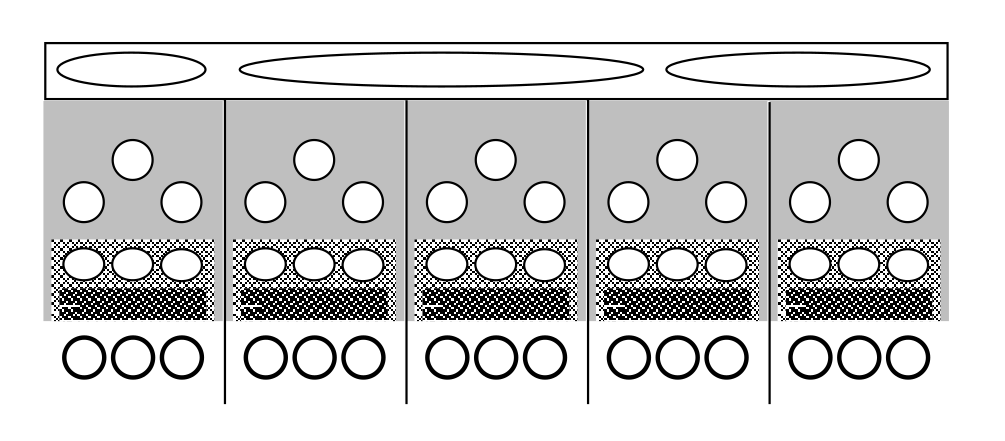
\includegraphics[scale=0.3]{hurricane}
      %%   \caption{Un système multi-cluster}
      %%   \label{fig:hurricane}
      %% \end{figure}
      %%
      Dans Hurricane, chaque cluster dispose de son propre ordonnanceur qui
      assure localement l’équilibrage de charge et l'ordonnancement des
      processus, tandis que l’équilibrage de charge inter-clusters est assuré
      par un ordonnanceur global. Les communications dans Hurricane peuvent être
      réalisées par l’envoi de messages ou par l’utilisation de Protected
      Procedure Calls (PPC).

      Un envoi de message est réalisé par l’interruption du cluster cible
      pour\benumline \item l’allocation d’un tampon mémoire pour réceptionner le
      message \item copier le message et les informations de contrôle depuis le
      processus émetteur du cluster source et \item attacher le tampon à la file
      d’attente du processus destinataire du message\eenumline.

      Quant un client demande un service, il change son espace d’adresse pour
      celui du serveur et invoque un thread de traitement associé à sa requête
      avant de retrouver son espace d’adressage initial.


    \subsubsection{Corey}

      Avant leurs travaux sur Linux,~\citet{boyd2008corey}. ont proposé le
      système d’exploitation Corey. Dans ce dernier, la gestion du partage des
      ressources est laissé aux applications utilisateurs.

      En donnant le contrôle aux programmeurs des applications utilisateur,
      Corey permet en effet de per- sonnaliser le comportement du noyau selon
      les besoins et les spécificités d’une application. Les inconvénients
      majeurs de cette approche sont: \benumline \item lier fortement l’application au
      système qui l’exécute, ce qui élimine complètement ou partiellement la
      portabilité des applications et complique sérieusement la réutilisation du
      code existant \item augmenter la complexité de programmation et
      nécessiter d’avantage d’efforts de la part des programmeurs d’applications
      (gestion explicite des régions virtuelles, placement et partage des
      structures de données noyau, etc.) et \item  générer des conflits entre
      les choix propres de chaque application dans le contexte de l’exécution
      dynamique de plusieurs applications simultanées\eenumline.


    \subsubsection{Barrelfish}
      
      L’ETH Zurich, en collaboration avec Microsoft Research, a engagé des
      travaux de recherches dans le domaines des architectures du futures en
      2008. Leur équipes sont arrivées à établir un nouveau modèle d’élaboration
      des systèmes d’exploitation : le
      multi-noyau~\citep{schupbach2008embracing}. Ce paradigme part de plusieurs
      postulats\benumline \item les architectures du futures seront très
      hétérogènes \item les noyaux actuels ne profite pas de l’hétérogénéité
      offertes par le matériel et au contraire essaye de la masquer un maximum
      \item les machines sont construites comme des systèmes distribués, pourquoi
        ne pas appliquer le même modèle aux systèmes d’exploitation\eenumline.

      \begin{figure}
        \centering
        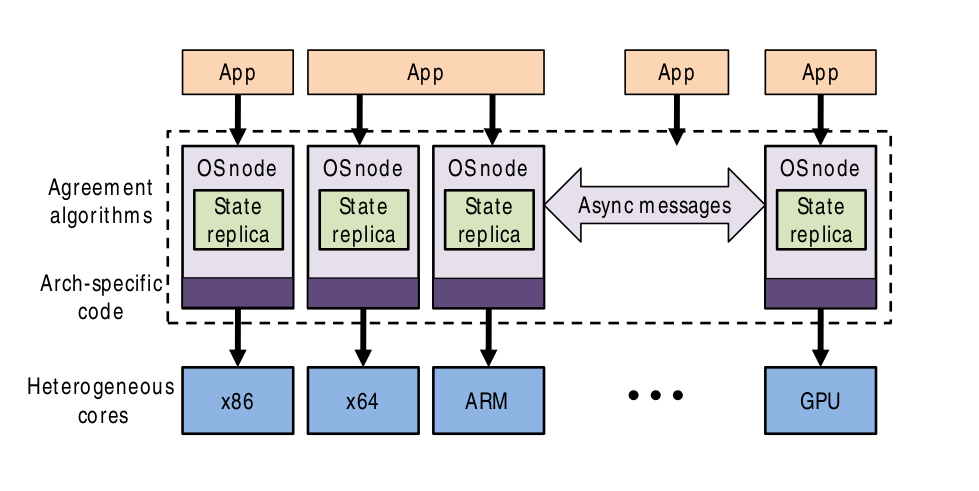
\includegraphics[scale=0.3]{barrelfish}
        \caption{L'architecture multi-noyau. Source:
          \citeauthor{schupbach2008embracing}}
        \label{fig:barrelfish}
      \end{figure}
        
      Selon l’approche multi-noyau (voir figure~\ref{fig:barrelfish}),
      l'environnement d’exécution des applications est une collection de n\oe
      uds où chaque n\oe ud est constitué d’un c\oe ur exécutant un OS à base
      d’un micro-noyau. Les communications entre les différentes OS se font par
      passage de messages : Barrelfish utilise une variante des Remote Procedure
      Calls au niveau utilisateur (URPC). chaque OS dispose d’un serveur système
      en mode utilisateur appelé Monitor. L’ensemble des moniteurs coordonnent
      collectivement l’accès à l’état global du système et maintient la
      cohérence des structures de données répliquées par c\oe ur (les tables
      d’allocation mémoire et les mappings des espaces d’adressages
      virtuels). La notion d’un processus dans Barrelfish est différente de
      celle d’un processus dans un noyau monolithique. Un processus est
      représenté sous formes d’un ensemble de Dispatchers avec un Dispatcher par
      c\oe ur où le processus peut être exécuté. Sur un c\oe ur, les Dispatchers
      sont ordonnancés par un ordonnanceur, au niveau du micro-noyau de ce c\oe
      ur, appelé CPU Driver. Ce dernier communique avec les Dispatchers (en mode
      utilisateur) à travers des up-calls.\newline
      

    \subsubsection{Influences}

      Bien que ces travaux n'apportent pas de réponses claires et définitives à
      notre problématique, il nous permettent de mieux comprendre les choix qui
      ont été fait dans le noyau ALMOS. Premièrement, les travaux sur Barrelfish
      ont apporté un nouveau modèle architectural pour la conception d'un
      noyau. Ce modèle semble cohérent et répond aux beoins des futures
      architectures. C'est donc le modèle qui a été retenu par
      ALMOS\footnote{Nous verrons plus en détail en section~\ref{sec:almos} le
        choix du multi-noyau.}. Néanmoins, Barrelfish ne respecte pas du tout
      les standards POSIX. C'est un choix très fort qui a été pour ce projet, et
      qui nous apparaît comme infondé.

      Les travaux sur Popcorn Linux, basé lui aussi sur le modèle du
      multi-noyau, ont permis de montrer que le noyau Linux, qui se veut être
      \textit{POSIX compliant}, peut être adapté à des architectures massivement
      parallèles, tout en respectant les normes. Le projet ALMOS, tout comme
      Popcorn Linux, a fait le choix d'avoir un système respectant au maximum
      les standards de conception des noyuax déja existants.

      Pourtant, ces recherches ne répondent pas à un des problèmes majeurs de
      l'architecture TSAR. En partant du principe que les processeurs
      d'aujourd'hui manipulent des informations sur 64 bits, les problèmes de
      gestion d'une grande quantité de mémoire ont été effacés. Nous allons tout
      de même présenter en section~\ref{sec:memory} quelques solutions
      permettant de contourner ce problème, mais toujours de manière incomplète.
    
     

  \subsection{Gestion des espaces d'adressage}
  \label{sec:memory}    

    \subsubsection{Les processeurs}

      MIPS registers\\
      PAE Intel


    \subsubsection{Linux, OpenBSD et NetBSD}
  
      Un des problèmes des espaces physiques de grande taille est la tables des
      descripteurs de pages physiques\footnote{L’utilisation du mot “table” est
        un abus de langage : dans les systèmes modernes, c’est en réalité une
        liste doublement chainée}. En effet, lors de l’initialisation du
      système, ce dernier crée tous les descripteurs de pages nécessaires pour
      décrire toute la mémoire physique de la machine~\citep{cranor1999uvm,
        gorman2004understanding}. Lorsque l’on dispose d’une grosse quantité de
      mémoire, la taille de cette table est énorme. A titre d’exemple, ALMOS à
      besoin de 14Go pour décrire les 1To de mémoire offerts par TSAR. Cette
      valeur, bien qu’élevée, est largement supérieure dans les noyaux Linux,
      OpenBSD et NetBSD, car les structures représentant les pages dans ces
      noyaux sont plus volumineuses en mémoire que celle d’ALMOS.

      Du fait de la taille énorme de ces descripeurs, le problème apparaît
      rapidement : comment stocker 14Go de données lorsque l’on a que 1Go
      d’espace virtuel ?  La réponse est simple : on ne peut pas.  Ainsi, les
      noyaux cités précédemment ne peuvent pas gérer plus de 4Go de mémoire dans
      leur versions 32 bits.


    \subsubsection{Le cas FreeBSD}

      Selon la documentation, il apparaît que le noyau de FreeBSD soit le seul
      capable de gérer une telle situation. Les développeurs indiquent que le
      noyau peut gérer jusqu’à 8To de mémoire, le tout en utilisant des tailles
      d’adresses de 32 bits~\citep{kernelfreebsd, mckusick1996design}.

      \todo{Je suis en train de voir ca sur une mailing-liste. Apparement il
        manquerait simplement un support MIPS pour certaines choses mais sinon
        ça devrait marcher (en tout cas pour la gestion d'1To de mémoire).}

      
  \subsection{Partage et maintient de cohérence de structures noyaux}
  \label{sec:consistency}
  
    %% \subsubsection{Hare}

    %% \subsubsection{Barrelfish}

    %%   passage de message

    %% \subsubsection{DragonFly BSD}

    %%   multi-noyau, passage de message, HAMMER
